


\documentclass[]{report}

\voffset=-1.5cm
\oddsidemargin=0.0cm
\textwidth = 480pt

\usepackage{framed}
\usepackage{subfiles}
\usepackage{graphics}
\usepackage{newlfont}
\usepackage{eurosym}
\usepackage{amsmath,amsthm,amsfonts}
\usepackage{amsmath}
\usepackage{enumerate}
\usepackage{color}
\usepackage{multicol}
\usepackage{amssymb}
\usepackage{multicol}
\usepackage[dvipsnames]{xcolor}
\usepackage{graphicx}
\begin{document}
	\section*{Question 32 - Backward Induction}
	
	\begin{figure}[h!]
\centering
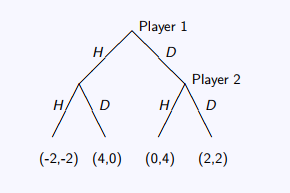
\includegraphics[width=0.5\linewidth]{Q32}
\caption{}
\label{fig:q32}
\end{figure}

\begin{itemize}
	\item Suppose Player 1 has played H. Player 2 obtains -2 by playing H
	and 0 by playing D. Hence, his best response to H is to play D.
\item Suppose Player 1 has played D. Player 2 obtains 4 by playing H
	and 2 by playing D. Hence, his best response to D is H.
\item Now we consider the action of Player 1.
%	37 / 45
%	Solution of Games with Perfect Information
\begin{itemize}
	\item If she plays H, then Player 2 will respond by playing D. Player 1
	obtains a reward of 4.
	\item If she plays D, then Player 2 will respond by playing H. Player 1
	obtains a reward of 0.
\end{itemize}

	\item It follows that Player 1 should play H. Player 2 follows by playing
	D.
	\item	The value of the game is (4, 0)
\end{itemize}
\section*{Question 32 - Translation to Extensive Form}
\begin{itemize}
	\item Since Player 1 has 2 strategies and Player 2 has 4 strategies, the
	payoff matrix will be of dimension 2 × 4.
\begin{itemize}	
\item   Player 1 can play H or D.
\item	Player 2 can play $(H|H, H|D)$, $(H|H, D|D)$, $(D|H, D|D)$ or
	$(D|H, H|D)$.
\end{itemize}
\begin{center}
\begin{tabular}{|c|c|} \hline
	$(H|H, H|D)$& Always be Hawk \\ \hline 
	$(H|H, D|D)$& Always do same as player 1 \\ \hline 
	$(D|H, D|D)$& Always be Dove \\ \hline 
	$(D|H, H|D)$& Alway do opposite as player 1\\ \hline 
\end{tabular}		
\end{center}
	We now consider the payoff vectors associated with each strategy
	pair.
	
\item Suppose Player 1 plays H.
\begin{enumerate}[(a)]
\item If Player 2 plays $(H|H, H|D)$ or $(H|H, D|D)$, 
    (\textit{i.e. always Hawk or alway the same}) then both players
	take the action H and the resulting payoff vector is (−2, −2).
\item If Player 2 plays $(D|H, D|D)$ or $(D|H, H|D)$
(\textit{i.e. always Dove or alway the opposite}), then Player 1
	takes the action H and Player 2 takes the action D and the
	resulting payoff vector is (4, 0).
\end{enumerate}
\item Now suppose Player 1 plays D.
\begin{enumerate}[(a)]
	\item If Player 2 plays ($D|H$, $D|D$) or $(H|H, D|D)$, 
	(\textit{i.e. always Dove or alway the same}) , then both players
	take the actions D and the resulting payoff vector is (2, 2).
\item If Player 2 plays $(H|H, H|D)$ or $(D|H, H|D)$,
   (\textit{i.e. always Hawk or alway the opposite}), then Player 1 takes
	the action D and Player 2 takes the action H and the resulting
	payoff vector is (0, 4).
	\end{enumerate}
\end{itemize}
\begin{figure}[h!]
\centering
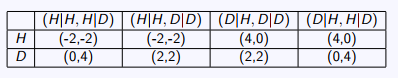
\includegraphics[width=0.7\linewidth]{Q32-matrix}
\caption{}
\label{fig:q32-matrix}
\end{figure}

\end{document}